    
\begin{minipage}{0.48\linewidth}
Une \textbf{pyramide} est un solide de l'espace qui a:
\begin{itemize}
\item Une base qui est un polygone.
\item Un autre sommet qui n'appartient pas à la base, appelé \og sommet principal \fg{}.
\item Les autres faces qui sont des triangles et qui ont tous en commun le \og sommet principal \fg{}.  
\end{itemize}
\end{minipage} 
\hfill
\begin{minipage}{0.48\linewidth}
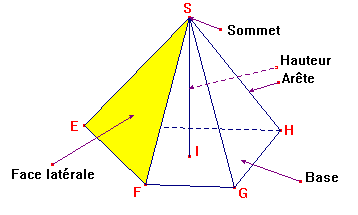
\includegraphics[scale=0.5]{RepS-pyramides_def.png}  
\end{minipage} 